
\renewcommand{\topfraction}{0.9}        % 允许页面顶部最多有 90% 的面积是图片
\renewcommand{\bottomfraction}{0.9}     % 允许页面底部最多有 90% 的面积是图片
\renewcommand{\textfraction}{0.1}       % 允许单页上文字最少只占 10%
\renewcommand{\floatpagefraction}{0.85} % 只有当图片占满页面的 85% 时，才允许它单独霸占一页

\chapter{雾天图像退化机理分析与数据集构建}
\label{chap:degradation_and_data}

海上无人机目标检测任务在复杂气象环境下具有重要的工程应用价值，其中雾天条件对视觉感知系统的影响尤为显著。雾气会引起图像对比度下降、边缘模糊以及细节信息衰减，从而导致检测模型对小尺度目标的识别能力显著下降。为了系统分析雾天退化对目标检测性能的影响机理，并为后续模型结构设计提供理论依据，本章从大气散射成像机理出发，对雾天图像的形成过程及其频率特性变化进行推导分析。在此基础上，引入小波多尺度分解理论，阐述其在雾天特征增强中的理论意义，并结合海上场景特点构建雾天数据集，为后续章节的模型改进与实验验证奠定理论与数据基础。

\section{大气散射成像机理与雾天图像退化分析}

在现代计算机视觉与物理光学交叉研究领域，为了从严谨的理论与数学物理角度定量解释并逆向求解雾霾等恶劣天气对光学传感器成像质量的退化影响，研究者们经过长期的观测与推导提出了经典的大气散射物理模型。该模型最早由麦卡特尼等人在研究大气层光辐射传播规律时建立，随后在计算机图形学与机器视觉领域被广泛引入并持续完善，现已成为单幅图像去雾任务理论建模、算法设计与逼真数据合成的核心基石。该模型从光辐射在参与介质中的传播机理出发，认为摄像机在雾霾等低能见度环境下接收到的成像信号由两类物理过程叠加形成：一类为目标表面反射光在传播过程中经大气衰减后到达成像设备的直接透射分量，另一类为环境光在大气介质中发生多次散射后进入摄像机的空气光分量。
\begin{figure}[!htbp]
    \centering
    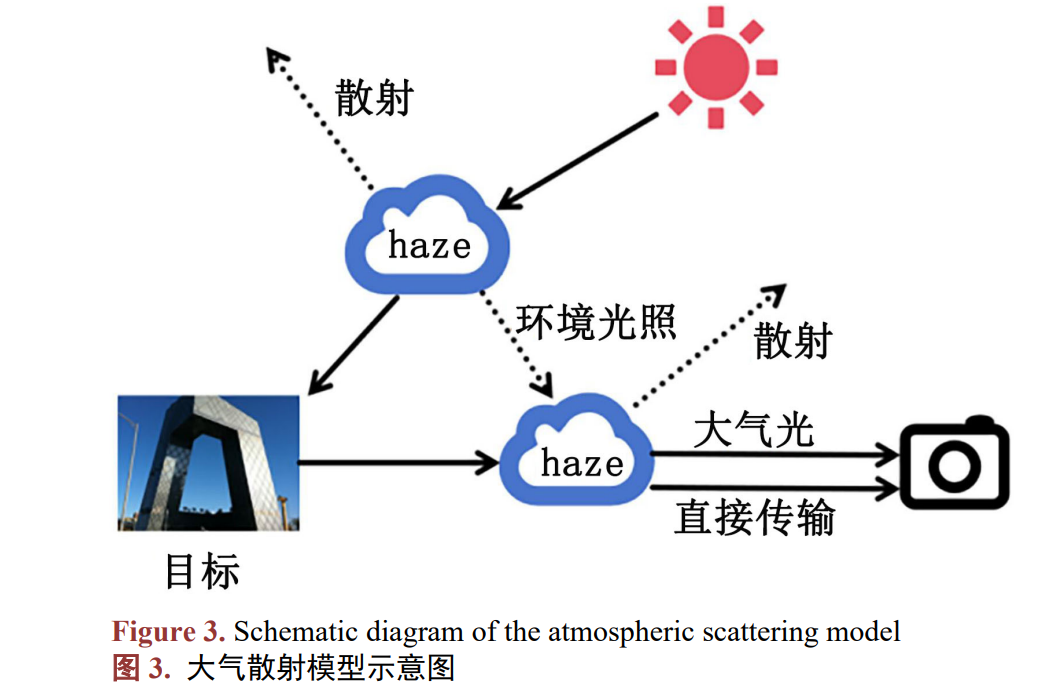
\includegraphics[width=0.9\linewidth]{figures/大气散射模型示意图.png}
    \caption{大气散射模型示意图}\label{Fig2-1}
\end{figure}

两者的线性组合构成雾天退化图像，其数学表达形式为
\begin{equation}
I(x) = J(x) t(x) + A (1 - t(x))
\label{eq:atmospheric_model_final}
\end{equation}

其中，$I(x)$ 表示观测到的退化图像，$J(x)$ 表示无雾条件下的真实场景辐射度，$A$ 为全局大气光强度，$t(x)$ 为透射率函数，用于描述光线在传播路径上未被散射而成功到达成像平面的能量比例。

根据朗伯–比尔定律，透射率与场景深度呈指数衰减关系：
\begin{equation}
t(x) = e^{-\beta d(x)}
\label{eq:transmission_final}
\end{equation}

式中，$\beta$ 为大气散射系数，用以刻画当前气象条件下悬浮颗粒的密度与散射能力；$d(x)$ 为场景深度，表示空间点到摄像机光学中心的距离。

由式(\ref{eq:transmission_final})可知，随着场景深度增加，透射率呈指数下降趋势。当 $d(x)$ 较大时，$t(x)$ 迅速趋近于零，直接透射分量显著衰减，而空气光分量逐渐占据主导地位。该物理机制在视觉层面表现为图像整体亮度上移、对比度压缩以及颜色偏移。对于海上无人机航拍场景而言，小尺度目标通常距离较远且在图像中所占区域有限，其透射率更低，因而更易受到空气光覆盖，导致目标与背景之间的亮度差异减弱，边缘信息模糊。

从空间梯度角度进一步分析，图像边缘与纹理信息可由强度函数的空间导数表示：
\begin{equation}
\nabla I(x) = \nabla \left[ J(x) t(x) \right]
\label{eq:gradient_final}
\end{equation}

在局部区域内，透射率 $t(x)$ 通常变化平缓，可近似视为低频平滑函数。因此，退化图像梯度主要受到乘性衰减项 $t(x)$ 的压缩作用，即
\[
\nabla I(x) \approx t(x)\nabla J(x)
\]

当 $t(x) < 1$ 时，图像梯度幅值整体下降，高频边缘响应显著减弱。由于深度卷积神经网络在目标检测过程中高度依赖局部梯度与纹理响应进行特征提取，上述物理退化机制将直接削弱网络对小尺度目标的判别能力，增加漏检与误检风险。

综上所述，大气散射模型揭示了雾天图像退化的本质机制：目标信号随传播距离指数衰减，而空气光分量以加性形式叠加于成像结果之中，二者共同导致对比度压缩与高频细节损失。该物理机制在远距离、小尺度目标场景下尤为显著，为后续去雾模型设计与雾天目标检测算法改进提供了理论基础。


\section{雾天图像的频率特性与小波分解理论}

在上一节基于大气散射模型分析了雾天图像在空间域中的物理退化机制之后，为进一步揭示雾气对图像结构信息的影响规律，本节将分析视角由像素空间域拓展至频率域。从数字信号处理理论出发，二维自然图像可以被视为不同频率、不同振幅二维基函数的线性叠加。频率分解为理解图像结构信息的分布与退化提供了更为本质的数学描述框架。

通常而言，图像的低频分量主要对应亮度缓慢变化的区域与大尺度结构信息，例如天空背景、平静海面及全局光照分布；高频分量则刻画物体边缘、纹理细节以及灰度剧烈变化的几何结构。在海上无人机远距离航拍场景中，落水人员、小型船舶等关键目标在整幅图像中所占像素比例极小，其判别信息主要集中于局部边缘与纹理响应之中，因此高度依赖高频特征表达。

结合式(\ref{eq:atmospheric_model_final})可知，雾天退化图像由乘性衰减项 $J(x)t(x)$ 与加性空气光项 $A(1-t(x))$ 共同构成。空气光分量在空间上变化缓慢，其频谱能量主要集中于低频区域，可视为一种低频增强项；而目标辐射分量中的高频细节则因透射率 $t(x)<1$ 的乘性衰减而整体压缩。由于透射率在局部区域内通常平滑变化，其频率成分亦偏向低频，因此不会补偿高频信息的损失。综合而言，雾天图像在频域层面呈现出显著的能量再分配现象：低频分量相对增强，高频分量显著衰减，频谱能量向低频区域集中。

这一频率重分布机制对小目标检测具有直接影响。深度卷积神经网络在特征提取过程中依赖局部梯度与纹理响应构建判别特征。当高频能量降低时，目标区域在特征图中的响应强度减弱，易被大面积低频背景掩盖。此外，常规网络结构中多层步长卷积或下采样操作会进一步压缩高频信息，使本已微弱的目标响应在传播过程中逐层衰减，从而增加漏检风险。因此，从频率补偿角度增强高频表达能力，是提升雾天小目标检测性能的重要理论方向。

为了在数学层面实现不同频率成分的有效分离与分析，小波变换提供了一种兼具空间定位能力与频率分解能力的时频分析工具。与全局傅里叶变换仅能提供频率分布而丧失空间位置信息不同，小波变换通过多分辨率分析框架，在保持空间局部性的同时完成频率分解，适用于非平稳信号的结构分析。
\begin{figure}[!htbp]
    \centering
    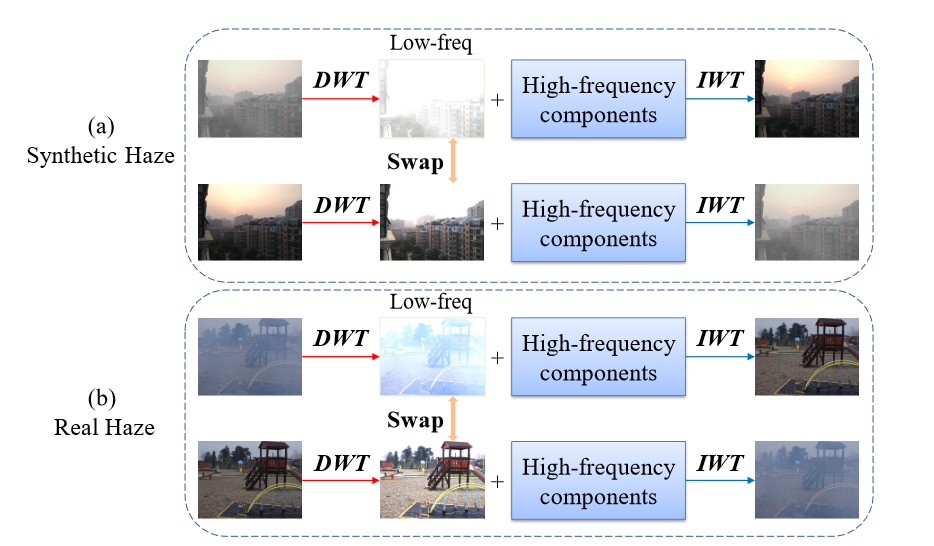
\includegraphics[width=0.9\linewidth]{figures/DWT实验.png}
    \caption{DWT实验}\label{Fig2-3}
\end{figure}

二维离散小波变换（Discrete Wavelet Transform, DWT）利用一组正交或双正交滤波器组，对图像进行一次分解后可得到一个低频近似子带和三个方向细节子带：
\begin{equation}
I(x,y) \rightarrow \{LL, LH, HL, HH\}
\label{eq:wavelet_final}
\end{equation}

其中，$LL$ 子带为低频近似分量，包含图像的主要轮廓与结构信息；$LH$、$HL$ 与 $HH$ 子带分别对应水平方向、垂直方向及对角方向的高频细节分量，用于刻画边缘与纹理结构。通过对 $LL$ 子带递归分解，可以构建多层级分辨率表示，实现对不同尺度结构的层次化分析。

在雾天退化图像中，由于高频响应整体减弱，$LH$、$HL$ 与 $HH$ 子带中的能量明显下降，而 $LL$ 子带则受到空气光低频增强效应的影响而占据更大能量比例。这种子带能量分布的不均衡性，从频率结构层面印证了上一节空间域分析所得出的结论：雾气在本质上通过增强低频分量并压制高频分量，破坏了目标的细节表达能力。

将小波分解嵌入特征提取框架具有两方面理论优势。首先，通过显式分离低频与高频子带，可以针对雾天退化特点对高频子带进行定向增强或补偿，从而恢复目标边缘与纹理信息；其次，小波分解所提供的层次化频率表示为跨尺度信息交互提供了清晰的结构基础，使不同尺度与不同方向的特征能够在保持空间分辨率的前提下进行融合与重构。

需要强调的是，小波分解并非单纯的频域变换操作，而是一种具有明确物理意义的结构分解方式。低频子带主要反映空气光与整体亮度结构，高频子带则对应目标几何边缘与局部纹理。当雾气作为低频掩膜覆盖图像时，其对高频子带的压制作用可以通过子带能量变化得到量化观测。因此，小波分析不仅为频率补偿提供技术手段，也为退化机理的数学解释提供验证工具。

综上所述，从频率视角分析可知，雾天退化的本质在于低频增强与高频衰减所引发的结构失衡。离散小波分解通过将图像表示为低频近似与方向性高频细节子带的组合，实现了对不同频率成分的可分离表达，为后续构建针对高频恢复与跨尺度信息交互的网络结构提供了理论支撑。


\section{基于物理先验的非均匀雾模拟方法}

在前述大气散射成像模型推导的基础上可以明确，雾天图像退化的物理本质来源于透射率的指数衰减机制与空气光分量的叠加效应。透射率与场景深度之间存在严格的负指数函数关系，该关系决定远距离区域在视觉层面呈现更强的遮蔽效应与对比度压缩现象。然而，在真实海洋环境中，大气悬浮颗粒的空间分布并不满足全局常数假设。受海面蒸发强度、温湿度梯度、局部气流扰动以及太阳辐射等因素影响，散射介质密度通常在空间上呈现连续变化趋势。因此，将散射系数视为常量的均匀散射模型难以刻画实际海面场景中的复杂退化结构。

为增强模型的表达能力，本文在经典大气散射框架内引入空间可变散射系数，将透射率函数推广为
\begin{equation}
t(x,y)=\exp\left(-\beta(x,y)\,d(x,y)\right)
\end{equation}
其中 $d(x,y)$ 表示像素对应的场景深度，$\beta(x,y)$ 表示空间变化的局部散射系数。该形式使退化强度同时受深度与局部气象扰动调制，从而形成更加符合物理现实的非均匀退化结构。

在非均匀透射率建模过程中，深度信息的获取构成关键前提。由于海上无人机影像通常仅具备单目输入形式，缺乏显式几何测量数据，本文采用预训练单目深度估计网络对清晰图像进行深度反演，获得初始深度场 $D_{raw}(x,y)$。该深度场可视为三维连续场景在二维图像平面上的尺度估计。然而，由于深度预测过程受到光照变化、海面高光反射以及网络泛化误差的影响，$D_{raw}(x,y)$ 在局部区域往往存在离群极值与断层跳变现象。若直接将该深度场代入指数衰减模型，极端值将导致透射率分布产生非物理性的剧烈波动。

为保证深度场在统计意义上的稳定性与连续性，首先对其进行分布约束。设深度矩阵的经验累积分布函数为 $F_D$，取其 $0.02$ 与 $0.98$ 分位数作为有效区间边界，构建截断算子
\begin{equation}
D_{clip}(x,y)=\max\left(P_{2},\min\left(D_{raw}(x,y),P_{98}\right)\right)
\end{equation}
该操作抑制由预测异常引发的尾部分布偏移，从而保证深度场满足有界性与有限方差假设。

在完成尾部分布约束后，为消除不同图像之间尺度不一致所带来的参数漂移问题，对截断后的深度场进行尺度标准化处理。设 $D_{min}$ 与 $D_{max}$ 分别为 $D_{clip}$ 的最小与最大值，则归一化映射为
\begin{equation}
D_{norm}(x,y)=\frac{D_{clip}(x,y)-D_{min}}{D_{max}-D_{min}+\epsilon}
\end{equation}
其中 $\epsilon$ 为防止分母为零的极小常数。该映射将深度值压缩至统一闭区间，使后续指数衰减参数具有明确物理含义。

为进一步提升空间连贯性，引入二维高斯卷积算子 $G_{\sigma}$ 对归一化深度场进行平滑处理：
\begin{equation}
D_{smooth}(x,y)=G_{\sigma} * D_{norm}(x,y)
\end{equation}
该平滑过程在频率域等价于低通滤波操作，可有效抑制高频振荡分量，从而避免透射率函数在空间域中产生非物理跳变。

在获得平滑深度先验 $D_{smooth}(x,y)$ 后，构建空间变化散射系数
\begin{equation}
\beta(x,y)=\beta_0 f(x,y)
\end{equation}
其中 $\beta_0$ 为全局雾强控制参数，$f(x,y)$ 为用于模拟局部气流扰动或高度梯度变化的调制函数。透射率计算形式为
\begin{equation}
t(x,y)=\exp\left(-\beta(x,y)D_{smooth}(x,y)\right)
\end{equation}
最终雾化图像由
\begin{equation}
I_{fog}(x,y)=J(x,y)t(x,y)+A\left(1-t(x,y)\right)
\end{equation}
给出，其中 $A$ 为全局空气光向量。由于透射率随深度单调递减，远距离区域自动获得更低透射率值，形成符合透视规律的非均匀遮蔽结构。

从频率角度分析，该模拟过程在空间域中实施指数衰减，在频域中表现为对高频分量的非线性压缩。结合前述小波多尺度分析理论，可以预期退化图像在高频子带中的能量显著下降，尤其在表示边缘与微小目标结构的方向性子带中表现明显。这一频率响应特性与真实雾天图像的统计规律一致，从而保证生成样本在多尺度表示空间内具备物理一致性。

\section{面向海上小目标检测的雾天数据集构建}

现有的公开的无人机小目标数据集信息如表\ref{tab:maritime_datasets}所示，主要分为真实数据集和合成数据集，数据集图例分别如图\ref{fig:real_datasets}、图\ref{fig:synthetic_datasets}所示。尽管现有公开数据集为无人机海上目标检测提供了宝贵资源，但它们在用于有雾条件下的目标检测模型训练时，存在以下几点核心局限性：

(1) 缺乏成对的有雾-清晰图像：绝大多数数据集（如SeaDronesSee、MOBDrone、Swimmers）都是在自然光照和晴朗天气下捕获的，没有针对有雾场景的图像，更没有与清晰图像成对的数据，而这种成对数据是训练去雾网络的先决条件。

(2) 雾气参数不可控：尽管一些合成数据集（如DGTA-SeaDronesSee、SynBASe）模拟了天气条件，但它们通常没有提供精细化的雾气参数，这导致我们无法系统性地控制和调整雾气强度，从而难以训练一个在不同雾天条件下都具有稳定鲁棒性的模型。

(3) 任务不一致：部分数据集（如Victims on Ocean、SynBASe）仅提供单一或有限类别的注释，无法满足多类别目标检测任务的需求。此外，这些数据集的设计目的并非去雾和检测的联合优化，因此无法为提出的两阶段流水线框架提供适用的训练和验证环境。

综上所述，为了克服现有数据集的局限性，并为去雾预处理和改进型RT-DETR模型提供高质量的训练和验证数据，构建一个包含可控雾气参数、成对有雾-清晰图像且具有精确标注的新数据集是本课题不可或缺的一环。

\begin{table}[!htbp]
\centering
\caption{海上小目标数据集}
\label{tab:maritime_datasets}
% \resizebox{\textwidth}{!}{ % 如果表格过宽，可取消此行和底部的 } 注释进行自动缩放
\begin{tabular}{lcccc}
\toprule
Dataset & Format  & Resolution & Images & Classes \\
\midrule
\multicolumn{5}{c}{Real (真实数据集)} \\
\midrule
SeaDronesSee & Img, Vid   & 1,280$\times$960 to 5,456$\times$3,632 & 54,000 & 5 \\
MOBDrone & Img, Vid   & 1,080$\times$1,080 & 126,170 & 5 \\
Swimmers & Img   & Up to 1,920$\times$1,080 & 9,000 & 1 \\
AFO & Img, Vid   & 1,280$\times$720 to 3,840$\times$2,160 & 3,647 & 6 \\
TinyPerson & Img   & 1,920$\times$1,080 & 1,610 & 3 \\
SeaPerson & Img   & 1,920$\times$1,080 & 12,032 & 3 \\
\midrule
\multicolumn{5}{c}{Synthetic (合成数据集)} \\
\midrule
DGTA-SeaDronesSee & Img  & 3,840$\times$3,840 & 100,000 & 5 \\
SynBASe & Img   & 1,200$\times$1,200 & 1,295 & 1 \\
Victims on Ocean & Img  & 512$\times$288 & 3,000 & 2 \\
\bottomrule
\end{tabular}
% }
\end{table}

\begin{figure}[!htbp]
    \centering
    % 第一张图
    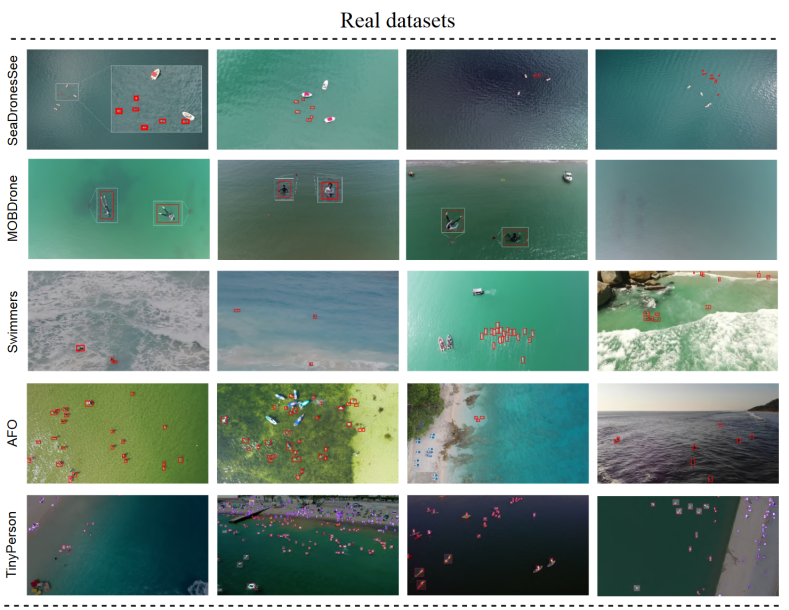
\includegraphics[width=0.7\linewidth]{figures/真实海上目标数据集图例.png}
    \caption{真实海上目标数据集图例}
    \label{fig:real_datasets}
    
    \vspace{1em} % 这里的 2em 用来手动控制两张图之间的垂直间距，您可以根据需要改大或改小
    
    % 第二张图
    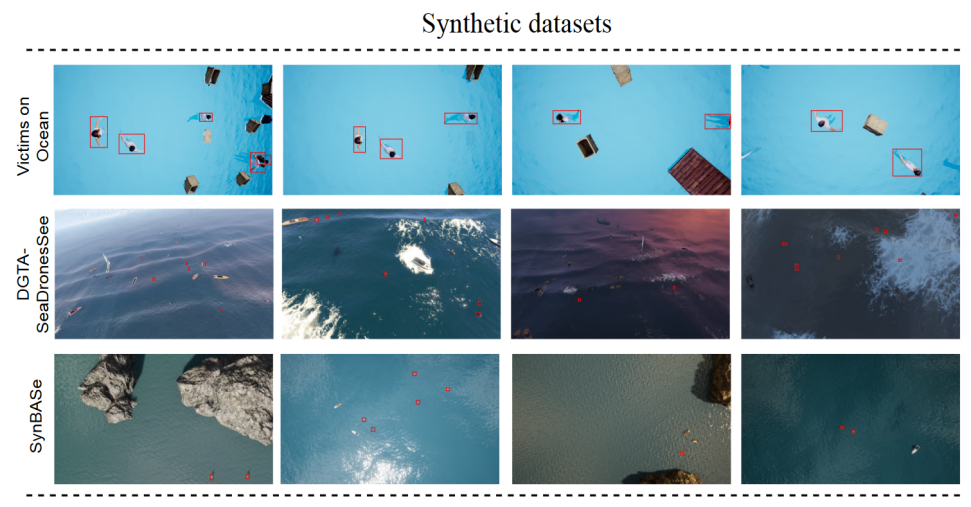
\includegraphics[width=0.7\linewidth]{figures/合成海上目标数据集图例.png}
    \caption{合成海上目标数据集图例}
    \label{fig:synthetic_datasets}
\end{figure}

于是在完成非均匀雾气模拟模型的理论构建后，本节围绕数据集的构建展开系统论述。数据集的目标在于为后续联合去雾与小目标检测模型提供具有物理一致性与统计代表性的训练与评估样本。原始数据来源于公开海上无人机航拍数据资源库。该数据集由50个真实无人机巡航视频片段构成，视频采集场景涵盖不同海域背景与气象条件。通过逐帧筛选与人工标注，共获得3647张高质量清晰图像样本，并包含39991个精确标注的小尺度海上目标实例。图像空间分辨率分布跨度从 $1280\times720$ 到 $3840\times2160$，覆盖主流工业级无人机成像规格。这种多分辨率分布为研究不同像素尺度下的退化影响提供了必要的统计基础。

在数据划分过程中，为避免模型对特定场景或飞行轨迹产生记忆偏置，采用基于视频片段的独立划分机制。训练集、验证集与测试集分别占样本总量的 $67.4\%$、$13.48\%$ 与 $19.12\%$。测试集样本来源于9个未参与训练与验证的独立视频片段。该划分方式在统计意义上构建了分布外评估条件，使模型性能能够在未见海域背景下进行客观验证。

在具体实现中，首先采用MiDaS模型对原始清晰图像进行单目深度估计。为了提升深度图的质量，减少网络预测中出现的局部噪声与跳变，采用归一化与高斯平滑操作对深度结果进行优化，从而保证雾效合成时的连续性与真实性，生成的深度图如图\ref{fig:depth_map_example}所示。随后，基于经典的大气散射物理模型，设置大气光照强度 $A=0.5$ 与散射系数 $\beta=0.01 \times i + 0.05$（其中 $i$ 为从 $0$ 到 $9$ 的整数），为每张清晰图像生成十个不同浓度等级的合成雾图。这种方法扩展了数据集的规模，使得每张清晰图像对应多种有雾条件下的变体，增强了训练数据的多样性与模型的泛化能力。原图以及生成的对应雾天图像如图\ref{fig:synthetic_fog_example}所示（以 $\beta=0.1$ 的浓度为例）。通过上述方法，本文构建了包含多雾浓度等级的扩展数据集，为后续去雾算法与检测算法的训练与客观评估提供了充分的数据支持。

\begin{figure}[!htbp]
    \centering
    % 请将此处替换为您真实的图片路径和文件名
    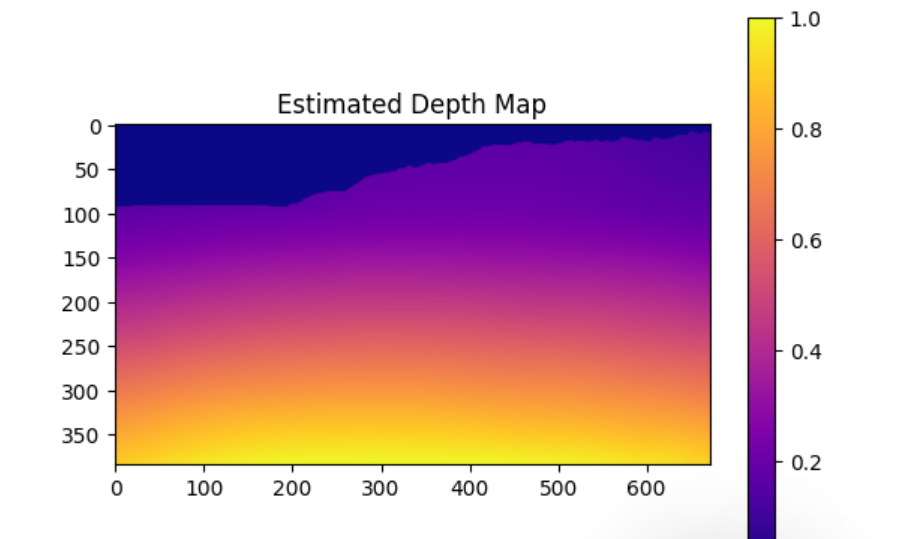
\includegraphics[width=0.7\linewidth]{figures/深度图.png}
    \caption{深度图示例}
    \label{fig:depth_map_example}
\end{figure}

\begin{figure}[!htbp]
    \centering
    % 请将此处替换为您真实的图片路径和文件名
    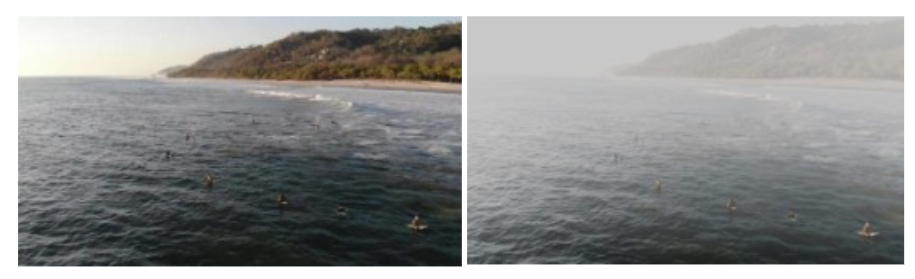
\includegraphics[width=0.8\linewidth]{figures/原图和合成雾天图像.png}
    \caption{AOF数据集原图（左）和模拟雾天图像（右）}
    \label{fig:synthetic_fog_example}
\end{figure}


由于雾化过程仅改变像素光度值而不引入几何变换，因此原始目标边界框坐标在雾化前后保持严格一致。清晰图像与退化图像在像素级实现一一对齐，为多任务联合训练提供稳定监督信号。从统计学习角度分析，该数据体系具备物理可解释性、连续退化梯度覆盖能力以及分布外测试机制。结合小波多尺度理论，可以进一步推断退化样本在高频子带能量分布上呈现系统性衰减趋势，而清晰样本保持较高频率响应。这种成对样本结构为后续构建频域增强机制提供了可量化监督基础。

综上，本节在物理模型约束下构建了具有空间渐变退化特性的海上雾天数据体系，并通过严格的统计划分机制确保其具备训练稳定性与评估可靠性。该数据体系在几何结构保持不变的前提下引入可控光度退化，为后续联合去雾与小目标检测模型设计提供了坚实的数据支撑。

\section{本章小结}
本章从底层的光学微观物理传播规律与图像多尺度时频信号交叉分析作为切入点，系统论证并详尽构建了全面支撑本文后续核心算法研究的理论基石与专用数据集工程体系。本章首先严密推导了经典的大气散射成像物理数学模型，从光度学指数级物理衰减的角度揭示了海上雾天无人机图像全局对比度下降与微小目标局部高频特征丢失的底层光学退化机理。随后引入离散小波高维分解频域分析理论，剖析了雾天退化图像的多尺度空间频率分布特性，在数学层面上明确指出了在深度神经网络架构中保留并定向增强原始高频细节信息对于微小目标高保真检测感知任务的不可替代性。在此理论指导下，本文详尽阐述了融合最新单目深度连续估计算法先验、通过异常分位数截断、线性归一化以及多维高斯低通平滑矩阵数值优化的海面物理非均匀雾气大规模模拟渲染核心算法。最后依托该鲁棒性的物理模拟流水线，本章成功地将现有的开源无雾航拍图像物理库转化为包含多梯度连续能见度气象条件且具备精确像素对齐成对边界框标注的专用海上雾天极小目标数据集。本章所涵盖的理论推导与底层数据工程实践开发，在根源上有效克服了复杂气象场景下真实物理成对视觉数据匮乏这一制约研究的工程障碍，更为后续即将展开的轻量级联合端到端特征检测深度算法的整体架构设计与底层模块优化提供了明确的物理指导原则与充实的数据验证基础。


本章从大气散射成像机理出发，系统分析了雾天环境下海上无人机图像的退化过程，指出透射率衰减与空气光叠加导致对比度压缩与高频细节衰减，是小目标检测性能下降的主要原因。进一步从频率角度分析了雾天图像能量分布变化规律，并引入小波多尺度表示理论，为后续特征增强结构设计提供理论支撑。同时构建了基于物理模型的非均匀雾模拟方法与数据体系，为模型训练与性能评估奠定基础。


